\chapter{General structure of the code}


\section{Equations to be solved}

\subsection{With dimensional variables}

We consider a lonely rotating star in a steady state. The star is
governed by the following equations for macroscopic quantities:

\begin{equation} \Delta\phi = 4\pi G\rho\end{equation}

\begin{equation} \rho T \vv\cdot\nabla s = -\Div\vF + \rho\eps_*\end{equation}

\begin{equation} \rho \vv\cdot\na\vv = -\na P -\rho\na\phi+\vF_v\end{equation}

\begin{equation} \Div(\rho\vv) =0\end{equation}
which need to be completed by the equations of microphysics:

\greq
P\equiv P(\rho,T)\\
\khi_r \equiv \khi_r(\rho,T)\\
\eps_* \equiv \eps_*(\rho,T)\\
\egreq
and the expressions of the viscous force, which could be (for instance)

\begin{equation} \vF_v = \mu(\Delta\vv + \frac{1}{3}\na\Div\vv)\end{equation}
for a compressible, constant viscosity fluid, and of the heat flux

\begin{equation} \vF = -\khi_r\na T -\frac{\khi_{\rm turb}T}{{\cal R}_M}\na s\end{equation}
where $\khi_{\rm turb}$ is the turbulent diffusion of heat and $s$ the
entropy.

This set of equations is completed by boundary conditions (discussed
below).

\subsection{Simplifications}

We simplify the system of equations by first neglecting entropy
advection by meridional circulation, which is justified at low viscosity
(e.g. \href{http://arxiv.org/abs/astro-ph/0608431}{\citealt{R06b}} or
\citealt{RELP16}).
We also neglect the convective flux: thus we avoid computing stars
with an outer convective envelope where the convective flux is
non-negligible. Core convection is simplified in assuming an isentropic
core. Hence, the energy/entropy equation just reads:

\begin{equation} -\Div\vF + \rho\eps_* = 0\end{equation}
in a radiative zone and

\begin{equation} \na s ={\vec 0}\label{nas}\end{equation}
in the convective core. This equation gives the temperature gradient as a function
of the pressure gradient thanks to the thermodynamics relation

\[ ds = \frac{c_p}{T}dT - \frac{\alpha_t}{\rho T}dP\]
where 

\beq \alpha_t = -\lp\frac{\partial \ln\rho}{\partial\ln
T}\rp_{\!\!P}\eeqn{alphat}
is the isobar expansion coefficient. Hence, \eq{nas} leads to

\begin{equation} \na T = \frac{\alpha_t}{\rho c_p}\na P\end{equation}
which also means that

\beq \nabla_a=\lp\frac{\partial \ln T}{\partial\ln P}\rp_{\!\!s} =
\frac{P\alpha_t}{\rho c_pT}\eeqn{nabla_ad}
As for the momentum equation, we split it into its azimuthal and
meridional components. The meridional components of the equation may be
reduced to

\begin{equation}
\rho s\Omega^2\es=\na p+\rho\na\phi
\label{baroc}
\end{equation}
where $s$ is the cylindrical radial coordinate \cite[e.g.][hereafter
referred to as ELR]{ELR13}. The vorticity equation reduces to

\begin{equation}
\label{eq:vort_inv}
s\frac{\partial\Omega^2}{\partial z}=\ephi\cdot\frac{\na
p\times\na\rho}{\rho^2} \;.
\end{equation}
In these equation, the advection of the 'meridian momentum' has been
neglected in view of the smallness of the meridional flow.

The meridian circulation is important in the advection of angular
momentum as it balances its diffusion by viscosity. So the $\ephi$
component of the momentum equation reads:

\begin{equation}
\label{eq:angular_mom}
\na\cdot{(\rho s^2\Omega\vu)}=\na\cdot (\mu s^2\na\Omega)
\end{equation}
where $\vu$ is the meridional circulation and $\mu$ the dynamical
viscosity.


\subsection{Scaled equations}

First step is to move scaled equations with scaled quantities. We choose
to scale pressure, density and temperature by their central values and
other quantities as follows:

\begin{center}\parbox{10cm}{

Length scale $\equiv$ polar radius \dotfill $R$

Pressure scale $\equiv$ central pressure \dotfill $P_c$

Density scale $\equiv$ central density \dotfill $\rho_c$

Temperature scale $\equiv$ central temperature \dotfill $T_c$

Gravitational potential scale \dotfill  $\frac{P_c}{\rho_c}$

Angular velocity scale \dotfill $\frac{1}{R}\sqrt{\frac{P_c}{\rho_c}}$

Meridional velocity scale \dotfill $E\sqrt{\frac{P_c}{\rho_c}}$
}
\end{center}\bigskip

\noindent where $E$ is the Ekman number defined as:

\begin{equation} E = \frac{\mu_c}{\rho_c \Omega_0 R^2} \with
\Omega_0=\sqrt{\frac{P_c}{R^2\rho_c}}\; .\end{equation}

With these scalings, the Poisson equation now reads:

\begin{equation} \Delta\phi = \pi_c \rho\end{equation}
where

\begin{equation} \pi_c = \frac{4\pi G\rho_c^2 R^2}{P_c}\label{picdef}\end{equation}
Energy equation can be written

\begin{equation} \Delta T + \na\ln\chi\cdot\na T +
\Lambda\rho\frac{\eps_*}{\chi_*} = 0\end{equation}
where

\begin{equation} \Lambda = \frac{\rho_c R^2}{T_c}\end{equation}
is a dimensional constant since $\eps_*$ and $\chi_*$ are dimensional. 

The momentum equation leads to

\begin{equation}
\rho s\Omega^2\es=\na p+\rho\na\phi
\label{baroc_nd}
\end{equation}
and the vorticity equation to

\begin{equation}
s\frac{\partial\Omega^2}{\partial z}=\ephi\cdot\frac{\na
p\times\na\rho}{\rho^2} \;.
\label{vort_nd}
\end{equation}
while angular momentum flux balance reads

\begin{equation}
\label{am_nd}
\na\cdot{(\rho s^2\Omega\vu)}=E\na\cdot (\mu s^2\na\Omega)
\end{equation}
Mass conservation remains the same

\begin{equation} \Div(\rho\vu) =0\end{equation}

\subsection{Boundary conditions}

Before presenting the boundary conditions, we should define the surface
of the star: we take as its definition, the isobar where the polar
pressure is 

\beq P_s=\tau_s\frac{g_{\rm pole}}{\kappa_{\rm pole}},\eeq
On this isobar, $T=T_{\rm eff}$ only at the pole. This definition
permits a smooth continuity with the non-rotating models. This surface
will be associated with the value $\zeta=1$ of the pseudo-radial
coordinate (see the chapter on the mapping).

\begin{itemize}
\item {\bf On the gravitational potential:} regularity at the centre of the
star and vanishing at infinity. However, imposing this condition on the
surface of the star is cumbersome and leads to problem of convergence
for very flattened stars. Different solutions to this problem are
possible. We can encompass the star within an empty
domain whose outer boundary is a sphere. On this outer sphere the
boundary conditions on spherical harmonics components of the
gravitational potential are simply

\[ 
\dr{\phi_\ell}+\frac{(\ell+1)\phi_\ell}{r}=0
\]
which ensure the matching with a field vanishing at infinity. This
solution was applied successfully in the first versions of the code but
is not appropriate when boundary conditions are implemented in real
($\theta$) space. We now prefer using an outer domain $\zeta\in
[1,+\infty[$ that is mapped to $[0,1[$ by an appropriate change of
variable (see chap. 6) so as to simply set the potential to zero on the
outer boundary of the encompassing outer domain.

\item {\bf On the velocity,} we demand stress-free conditions, namely

\[ \vv\cdot \vn =0 \quad {\rm and}\quad ([\sigma]\vn)\wedge\vn =\vzero
\]
where $[\sigma]$ is the stress tensor. Stars are in the limit of
small Ekman numbers and it is interesting (numerically) not to have to
compute the ensuing Ekman layer. However, it is necessary to take this
layer into account for computing the azimuthal velocity, which
is otherwise undefined (see ELR).
ELR have shown that the effect of the Ekman layer on
the interior flow can be mimicked by the boundary condition:

\begin{equation}
\label{eq:bl}
\mu
s^2\vec{\hat\xi}\cdot\na\Omega+\psi\vec{\hat\tau}\cdot\na(s^2\Omega)=0
\qquad\mbox{on the surface}\;.
\end{equation}
where $\vec{\hat\xi}$ is a unit vector perpendicular to the surface
while $\vec{\hat\tau}$ is tangent to it. $\psi$ is the stream
function of the meridional flow.

\item {\bf The rotation speed} of the star must be specified. For this we
impose the equatorial angular velocity as a fraction of the critical
angular velocity, namely:

\[ \Omega(r=R_{\rm eq},\theta=\pi/2) =
\omega_k\sqrt{\frac{GMR^2\rho_c}{P_cR_{\rm eq}^3}}\]
where $\omega_k$ is chosen by the user. Another way of specifying the
angular velocity of the star is to impose its total angular momentum
(see integral constraints).

\item {\bf On temperature:} with the adopted definition of the stellar surface
and thanks to a simple model described in ELR, we can ascribe
to the surface of the star a temperature profile, such that

\beq T_b(\theta) = \lp\frac{g_{\rm pole}}{g_{\rm
eff}(\theta)}\frac{\kappa(\theta)}{\kappa_{\rm
pole}}\rp^{1/(n+1)}\lp\frac{-\khi_r\vn\cdot\na T}{\sigma}\rp^{1/4}\;.
\eeqn{tb}
where the polytropic index $n$ is set to $n=3$. So the temperature
boundary condition are simply:

\[ T(0) = 1 \andet T(\zeta=1,\theta)=T_b(\theta)/T_c\]


\end{itemize}

\subsection{Integral constraints}

\begin{itemize}
\item Mass is an input parameter that is related to the preceding
quantities by

\beq M = \rho_cR^3\intvol \rho dV = \rho_cR^3 m\eeqn{massdef}

\item Angular momentum is another integral quantity that is useful to
monitor or to impose:

\beq L = \rho_cR^4\sqrt{\frac{P_c}{\rho_c}}
\intvol r^2\sin^2\theta\Omega\rho dV \eeq

\end{itemize}

\subsection{The mapping}

The foregoing equations and boundary conditions should be completed by
the definition of the mapping that maps the spheroidal star to a sphere.
This thorny subject is described at length in a separate chapter
(see chap.~\ref{chap:mapping}).

\section{The algorithm}

\subsection{Discretization}

This system of partial differential equation is solved using a spectral
method or more precisely spectral elements. The star divided in
``onion" layers where the vertical direction is discretized on the
Gauss-Lobatto collocation grid (associated with Chebyshev polynomials)
and the Gauss-Legendre collocation grid for the horizontal dependence.
This is associated with Legendre polynomials (or axisymmeric spherical
harmonics).

Let us recall the ordering of pressure discretized values, namely

\[\begin{array}{cccc}
p(\zeta_0,\theta_0)&p(\zeta_1,\theta_0)&p(\zeta_2,\theta_0)&\cdots\\
p(\zeta_0,\theta_1)&p(\zeta_1,\theta_1)&p(\zeta_2,\theta_1)&\cdots\\
p(\zeta_0,\theta_2)&p(\zeta_1,\theta_2)&p(\zeta_2,\theta_2)&\cdots\\
\vdots&\vdots&\vdots&
\end{array}\]
Scalar fields can therefore be represented by a 2D matrix

\[ p_{ij}\]
where the first index represents the radial variations and the second the
angular variations. Hence, operators acting on $\zeta$ apply on "left"
while operators acting on $\theta$ apply on right of the matrix $[p]$.
Hence, we shall write

\[ [\partial_{\zeta\theta}p] = [D_\zeta][p][D_\theta]\]
or

\[ (\partial_{\zeta\theta}p)_{ij} = (D_\zeta)_{ik}p_{kl}(D_\theta)_{lj}\]


\subsection{Iterations}

We solve the resulting discretized equations using Newton's iterative
scheme, namely, if  we write the problem in the form

\begin{equation}
\vec F(\vec x)=\vec 0 ,
\end{equation}
where the vector function $\vec F$ represents the equations that we
want to solve and $\vec x$ is the vector containing all the independent
variables of the problem (pressure, temperature, \ldots) including the
shape of the surface which is not known a priori.  The equations are
linearized using the Jacobian matrix $\tens J$ of $\vec F(\vec x)$ such
that

\begin{equation}
\delta\vec F(\vec x)=\tens J (\vec x) \delta\vec x .
\end{equation}
The correction to the solution $\delta \vec x^{(k)}$ at the $k$-th
iteration is calculated solving the linear system

\begin{equation}
\tens J(\vec x^{(k)})\delta \vec x^{(k)}=-\vec F(\vec x^{(k)})
\end{equation}
and the solution is updated with
$\vec x^{(k+1)}=\vec x^{(k)}+\delta \vec x^{(k)}$.

With an appropriate initial approximation $\vec x^{(0)}$, Newton's method
has quadratic convergence. In practice, a rotating stellar model can be
calculated in approximately 10 iterations starting with the corresponding
non-rotating model.

\section{Implementation}

\subsection{The vector}

The solution vector $\vx$ is built from the discretized variables as
follows

\begin{table}
\begin{center}
\begin{tabular}{lcll}
\hline
Variable & Dependence & C++ quantity & Comments \\
\\
$\phi$   & $(\zeta,\theta)$ &  Phi & Gravitation potential \\
$\ln P$  & $(\zeta,\theta)$ &  log\_p & Natural log of pressure     \\
$\ln T$  & $(\zeta,\theta)$ &  log\_T & Natural log of temperature  \\
   w     &  $(\zeta,\theta)$ &   w  & Differential Rotation    \\
$\psi$   &  $(\zeta,\theta)$ &   G  & Stream function    \\
$T_{\rm eff}$ & $\theta$ &  Teff  &  Effective temperature  \\
$g_{\rm sup}$ & $\theta$ &  gsup  &  Effective surface gravity  \\
$P_s$    &  $\theta$  &ps    &  surface pressure \\
$T_s$    &  $\theta$  &Ts    &  surface temperature \\
$\gamma$ &  $\theta$    & gamma    &
$\gamma=\sqrt{g^{\zeta\zeta}}=\sqrt{1+r_\theta^2/r^2}$ at the surface \\
$F_{\rm rad,i}$ &  $(\theta, i)$ &  Frad & $\vF_\zeta$ Radiative flux
component at each domain boundary\\
$R_i$    &  $(\theta,i)$       &   Ri & boundaries of the domains \\
$dR_i$   &  $(\theta,i)$       &   dRi& $R_{i+1}-R_i$      \\
$\eta_i$ &                   &   eta& Polar radius of the domains \\
$d\eta_i$&                   &  deta& $\eta_{i+1}-\eta_i$      \\
$\pi_c$  &                  &  pi\_c &  Non-dimensional central pressure \\
$\Lambda$&                  &  Lambda &   Dimensional constant  \\
$\Omega$ &                  &  Omega  &   Equatorial angular velocity \\
$\ln P_c$&                  & log\_pc &   log of central pressure  \\
$\ln T_c$&                  & log\_Tc &   log of central temperature  \\
$\log R$ &                  &log\_R  &   log of polar radius \\
$m$      &                  &       m     & non-dimensional mass\\
Lum      &                  &  lum   &  Luminosity  \\
      \hline
\end{tabular}
\end{center}
\caption[]
{This table lists all the primary variables contained in $\vx$ but not
in their actual order in the code.}
\end{table}

\begin{table}
\begin{center}
\begin{tabular}{lll}
\hline
C++ Variable & Dependence (C++ quantity) & Comments \\
\\
T  & log\_T & Temperature \\
r  & R$_i$, dR$_i$, $\eta_i$, d$\eta_i$      & radius \\
rz &    R$_i$, dR$_i$, $\eta_i$, d$\eta_i$   & $\partial_\zeta r$\\
log\_rhoc &   log\_pc,log\_Tc   & log of central density \\
rho &   log\_T,log\_p    & density \\
opa.xi &   log\_T,log\_p    & thermal conductivity \\
opa.k &   log\_T,log\_p    & opacity \\
nuc.eps &   log\_T,log\_p    & nuclear heating \\
s  &   log\_T,log\_p    & entropy \\
\hline
\end{tabular}
\end{center}
\caption[]
{This table lists all the secondary variables. They depend on the
primary variables and are used as short-cut in the programming.}
\end{table}





\noindent Real ordering of variables:

"Phi"; "log\_p"; "pi\_c"; "log\_T"; "Lambda"; "eta"; "deta"; "Ri";
"dRi"; "Omega"; "log\_pc"; "log\_Tc"; "log\_R"; "m"; "ps"; "Ts"; "lum"; "Frad"; "Teff"; "gsup"; "w"; "G"; "gamma"; 

\subsection{The equations}

\subsubsection{$\bullet$ \bf Initialization {\tt fill}}

Uses \eq{massdef} and that

\[ m=2\pi\int_0^1\int_0^\pi\rho r^2r_\zeta d\zeta\sin\theta d\theta\]
Set the definition of $\pi_c$ as \eq{picdef}, and the definition of 
$\Omega_c$, namely the scaled keplerian velocity. We have

\[ \Omega_c=\frac{\Omega_k}{\Omega_0} \with \Omega_k=\sqrt{\frac{GM}{R_e^3}}\]
and $\Omega_0^2=P_c/\rho_c/R^2$.

\subsubsection{$\bullet$ \bf Constitutive relations {\tt solve\_definitions}}

Secondary variables are used to simplify the writing of the Jacobian
matrix.

The EOS is written as the dependence of $\rho_*$ with respect to $P_*$ and
$T_*$ ($*$ quantities are dimensional). Thus we have:

\[ \delta\rho_* = \frac{\rho_*}{P_*}\lp\frac{\partial\ln\rho}{\partial\ln
P}\rp_T\delta(P_cP) + \frac{\rho_*}{T_*}\lp\frac{\partial\ln\rho}{\partial\ln
T}\rp_P\delta(T_cT)\]
After some manipulations, we get:

\[ \frac{\delta\rho}{\rho} = \frac{1}{\chi_\rho}\delta\ln P +
\frac{1}{\chi_\rho}\delta\ln P_c -\delta\ln\rho_c - d_p\delta\ln T_c -
d_p\delta\ln T\]
where we introduced

\[ \chi_\rho = \lp\frac{\partial\ln P}{\partial\ln\rho}\rp_T \andet d_p
= -\lp\frac{\partial\ln\rho}{\partial\ln T}\rp_P = \chi_t/\chi_\rho \]
following the definitions of \cite{RSI96} and using the thermodynamic
triangular relation.

\bigskip
Opacity and nuclear heat production depend on $\rho$ and $T$. So for both of
these quantities we have the formal relation $f=f(\rho,T)$. For instance, for
opacity, denoted $\kappa$ we get

\[ \delta\kappa = \frac{\partial\kappa}{\partial\rho_*}\delta\rho_* +
\frac{\partial\kappa}{\partial T_*}\delta T_*\]
Noting that $\rho_*=\rho_c\rho$ and $T_*=T_cT$, after some manipulations we
get:

\[ \delta\kappa =
\frac{\kappa}{\rho}\frac{\partial\ln\kappa}{\partial\ln\rho}\delta\rho +
\kappa\frac{\partial\ln\kappa}{\partial\ln\rho}\delta\ln\rho_c +
\kappa\frac{\partial\ln\kappa}{\partial\ln T}\delta\ln T +
\kappa\frac{\partial\ln\kappa}{\partial\ln T}\delta\ln T_c\]
For radiative conductivity, its expression

\[ \chi = \frac{16\sigma T^3}{3\rho\kappa}\]
leads to the following contribution

\[ \frac{\delta \chi}{\chi} = 3\delta\ln T+3\delta\ln T_c
-\frac{1}{\rho}\delta\rho - \delta\ln\rho_c - \frac{1}{\kappa}\delta\kappa\]
where we took into account that $\rho$ and $T$ are non-dimensional.

As far as entropy is concerned, we express its dependence with temperature and
pressure:

\[ \delta s = \frac{c_p}{T_*}\delta T_* + \lp\frac{\partial s}{\partial
P_*}\rp_T\delta P_*\]
We note that

\[ \lp\frac{\partial s}{\partial
P_*}\rp_T = -\frac{\alpha}{\rho} = -\frac{c_p\nabla_a}{P}\]
where we used \eq{alphat} and \eq{nabla_ad}.
Thus, after some manipulations we find

\[ \delta s = c_p\lp\delta\ln T_c + \delta\ln T - \nabla_a\delta\ln P_c
-\nabla_a\delta\ln P \rp\]

\subsubsection{$\bullet$ \bf Poisson equation {\tt solve\_poisson}}

Poisson equation reads

\[ \Delta \phi = \pi_c \rho \qquad {\rm with}\quad  \pi_c = \frac{4 \pi G
\rho_c^2 R^2}{p_c}\]
so that its variational expression is 

\[ \Delta \delta\phi +(\delta\Delta)\phi - \rho\delta\pi_c  -
\pi_c\delta\rho = -(\Delta \phi - \pi_c \rho)_n \]
where $(\delta\Delta)$ represents the variation of the Laplacian operator due
to the change of the metric. Note that the last domain is void of matter.

Together with Poisson equation, we need to impose the boundary conditions and
the interface conditions at each domain boundary. The boundary conditions are

\[ \na\phi(\vzero) = \vzero  \andet \phi(\infty) = 0\]
The first condition is equivalent to $\partial_\zeta\phi=0$.

At the interface of the domains we demand that $\phi$ and $\vn\cdot\na\phi$
are continuous. The continuity of the normal component of the gradient implies
the continuity of

\[ \frac{1}{r_\zeta}\dzeta{\phi}\]
Even though we have chosen a continuous $r_\zeta$-field, we keep the
dependence of the interface condition with $r_\zeta$ in case we would like to
test other kinds of mapping (see chapter 6 for more details).

\subsubsection{$\bullet$ \bf Momentum equation {\tt solve\_mov}}

We start from the meridional components of the (inviscid) momentum equation
\eq{baroc_nd}, \eq{vort_nd} and \eq{am_nd}. For the angular momentum
equation \eq{am_nd}, we impose boundary condition \eq{eq:bl}.

The equation are solved for the log of the pressure. At the domain
interfaces we impose the continuity of pressure, while at the center the
non-dimensional pressure is set to unity.

Let us discuss the implementation of the vorticity equation. We first rewrite \eq{baroc_nd} as 

\[ \na p +\rho\na\phi -\rho s\Omega^2\es=\vzero\]
and introduce the {\tt eqmov} equation as

\bigskip
\centerline{\tt eqmov=grad(p)+rho*grad(phi)-rho*s*w*w*svec;}
\bigskip
\noindent from which we derive the equation of vorticity \eq{vort_nd}, symbolically name {\tt eq\_vort},
and defined as

\centerline{\tt eq\_vort=(phivec,curl(eqmov/rho));}
\bigskip
\noindent which means the scalar product of $\ephi$ with the curl of
the equation {\tt eqmov} by $\rho$.

At the interface of the domain, since we are working in the inviscid
limit, $\Omega$ is not necessarily continuous. It is continuous only if
$\rho$ is continuous (see discussion in \citealt{ELR13}). In general we
only know that pressure is continuous and so is its horizontal
derivative. Thus the continuity of $\Omega$ is ruled by the continuity
of the horizontal component of $\rho\na\phi-\rho s\Omega^2\es$ as
explained by Eq. (63) in \cite{ELR13}. Thus the programme introduces:

\bigskip
\centerline{\tt ic\_w=covariant(eqmov-grad(p))(1);}
\bigskip
\noindent namely the $\theta$ (as 1) covariant component of $\rho\na\phi-\rho s\Omega^2\es$,
since $\vE_\theta$ is parallel to $\zeta=\cst$ surfaces.
\bigskip

The vorticity equation, which is called "w", is then plugged into the
big Jacobian matrix by just saying that  functional variations are on
variables "p", "w", "rho" and "r" like

\begin{center}
{\tt
        eq\_vort.add(op,"w","p");\qquad eq\_vort.add(op,"w","w"); \par
        eq\_vort.add(op,"w","rho"); \qquad eq\_vort.add(op,"w","r"); \par
        op->set\_rhs("w",-eq\_vort.eval()); \par
}
\end{center}
Equation "w" is completed by the interface and boundary conditions that
say that:

\[ \partial_\zeta\Omega(\zeta=0) = 0,\quad {\rm at\; center} \]

\[ \mu s^2\vn\cdot\na\Omega +
G\vec{t}\cdot\na(s^2\Omega)=0,\quad {\rm at\; surface} \]
\[ \Omega(\zeta=1,\theta=\pi/2) = \Omega_e\]
where $G$ is the stream function $\psi$ in \eq{eq:bl}.
The central boundary condition reads:
\bigskip

\centerline{\tt
op->bc\_bot2\_add\_l(0,"w","w",ones(1,nth),D.block(0).row(0));}
\bigskip

Then we loop on the domains to impose the continuity of {\tt ic\_w}

\begin{center}
{\tt
        for(int n=0;n<ndomains-1;n++) \{  \par
                ic\_w.bc\_top1\_add(op,n,"w","w");  \par
                ic\_w.bc\_top1\_add(op,n,"w","rho");  \par
                ic\_w.bc\_top1\_add(op,n,"w","Phi");  \par
                ic\_w.bc\_top1\_add(op,n,"w","r");  \par
                ic\_w.bc\_top2\_add(op,n,"w","w",-ones(1,nth));  \par
                ic\_w.bc\_top2\_add(op,n,"w","rho",-ones(1,nth));  \par
                ic\_w.bc\_top2\_add(op,n,"w","Phi",-ones(1,nth));  \par
                ic\_w.bc\_top2\_add(op,n,"w","r",-ones(1,nth));  \par
                rhs.setrow(j0+map.gl.npts[n]-1,  \par
-ic\_w.eval().row(j0+map.gl.npts[n]-1)+ic\_w.eval().row(j0+map.gl.npts[n]));\par
  \par
                j0+=map.gl.npts[n];  \par
        \}  \par
}
\end{center}

\bigskip
Then we impose the condition on the value of the velocity at equator and
the special BC that suppresses the Ekman layer:
\eq{eq:bl} is inserted as

\bigskip
\centerline{\tt
bc=mu*s*s*(nvec,grad(w))+G*(tvec,grad(s*s*w));
}

\bigskip
\noindent and plugged in the BC of the last domain. So the outer
boundary condition on $\Omega$ imposes the angular velocity at
equator. Since $\Omega$ obeys a first order equation the central
condition and its fixed equatorial value determines $\Omega$ everywhere
provided we lift the degeneracy $\Omega^2\tv\Omega^2+f(s)$ where $f$ is
arbitrary. This is done by \eq{eq:bl} which also provides the second BC
for $G$ the stream function which obeys a second order PDE. Hence,
noting that $\Omega_{\rm eq}$ is a linear function of the values of
$\Omega$ on the latitudinal grid, BC \eq{eq:bl} is imposed on all the
grid points except the first one where the equatorial angular velocity
is imposed: hence,

\bigskip
\begin{center}
{\tt
        q=ones(1,nth);  \par
        q(0)=0;  \par
        map.leg.eval\_00(th,PI/2*ones(1,nth),TT);  \par
        bc.bc\_top1\_add(op,ndomains-1,"w","G",q);  \par
        bc.bc\_top1\_add(op,ndomains-1,"w","w",q);  \par
        bc.bc\_top1\_add(op,ndomains-1,"w","rho",q);  \par
        bc.bc\_top1\_add(op,ndomains-1,"w","r",q);  \par
        op->bc\_top1\_add\_r(ndomains-1,"w","w",(1-q),TT);  \par
        op->bc\_top1\_add\_d(ndomains-1,"w","Omega",-(1-q));  \par
        rhs.setrow(-1,-q*bc.eval().row(-1)-(1-q)*((w.row(-1),TT)-Omega));  \par
        op->set\_rhs("w",rhs);  \par
}
\end{center}

Of course the equation for $\Omega$ is strongly coupled to that of the
meridional circulation that is represented by the stream function $G$,
which is actually the stream function of $\rho\vv$. Hence, one introduces

\centerline{\tt V=curl(G*phivec)/rho;}
\bigskip
\noindent namely the meridional circulation, and the angular momentum equation:

\bigskip
\centerline{\tt  eq\_phi=div(rho*s*s*w*V)-div(mu*s*s*grad(w));}
\bigskip

Again the equation of angular momentum is plugged into the Jacobian
matrix by:

\bigskip
\begin{center}
{\tt
        eq\_phi.add(op,"G","w");  \par
        eq\_phi.add(op,"G","G");  \par
        eq\_phi.add(op,"G","rho");  \par
        eq\_phi.add(op,"G","r");  \par
        op->set\_rhs("G",-eq\_phi.eval());  \par
}
\end{center}
\bigskip
Then it is indicated that $G$ is zero at the center and continuous at
the interfaces.







For non-dimensional parameters like $\pi_c$, it is continuous at the domain
interface:

\[ 1\times\delta\pi_c({\rm 1}) -1\times\delta\pi_c({\rm 2}) = 0\]
``1" means ``part 1 of the interface condition" and ``2" means ``part 2
of the interface condition" (see Fig.~\ref{matp}).


\subsubsection{$\bullet$ \bf Temperature equation {\tt solve\_temp}}

First, the luminosity at each domain boundary is computed through

\[ L_n = 2\pi\Lambda\int_0^\pi\int_0^{\eta_n} \rho\eps_* r^2r_\zeta\sth
d\theta\]
The definition of the luminosity 

\[ L=\Lambda\intvol \rho\eps_* dV \with \Lambda = \frac{\rho_cR^2}{T_c}\]
is differentiated and yields

\[ \delta L - \Lambda\intvol (\delta\rho\eps_* +\rho\delta\eps_*)dV -
\delta\Lambda\intvol \rho\eps_* dV - \Lambda\intvol \rho\eps_* \delta dV
= 0\]
with $L$ continuous at domain interfaces.

Then we introduce

\[ \frad = -\chi\vE^\zeta\cdot\na T\]
so the projection of the radiative flux on $\vE^\zeta$, the normal
direction of the $\zeta=\cst$ surfaces ($\chi$ is the thermal
conductivity). The basic property of this
scalar quantity is that it gives the radiative luminosity when
integrated over a surface, namely

\[ L= \intsur \frad dS\]
where

\[ dS = 2\pi r^2r_\zeta\sth d\theta\]
Explicit expression of $\frad$ is

\[ \frad = \chi\lp\gzz\partial_\zeta T + \gzt\partial_\theta T \rp\]
so that the functional derivative is given by

\[ \delta\frad -\frac{\frad}{\chi}\delta\chi -\chi\lp
\gzz\partial_\zeta\delta T + \gzt\partial_\theta\delta T +
\delta\gzz\partial_\zeta T + \delta\gzt\partial_\theta T\rp = 0\]
where we have

\[ \delta\gzz = -2r(\gzt)^2\delta r -\frac{2\gzz}{\rz}\delta\rz
-\frac{2\gzt}{\rz}\delta r_\theta\andet
\delta\gzt = -\frac{2\gzt}{r}\delta r -\frac{\gzt}{\rz}\delta\rz
-\frac{\delta r_\theta}{r^2\rz}\]

Then we introduce the masks of the convective zones (CZ) {\tt qconv} and
of the radiative zones (RZ) {\tt qrad}.

\[ {\tt qconv}(\vr) = 1 \qquad {\rm if}\quad \vr \in {\rm CZ}\]
\[ {\tt qrad}(\vr) = 1 \qquad {\rm if}\quad \vr \in {\rm RZ}\]
and of course {\tt qconv+qrad=1} $\forall \vr$.

Hence, the temperature equation can be written

\beq q_{\rm conv}(\vn\cdot\na s) +  q_{\rm rad}\lp\frac{\Div(\chi\na
T)}{\chi} + \Lambda\rho\frac{\eps_*}{\chi_*}\rp = 0\eeqn{eq_temp}
where $\vn$ is the unit vector opposite to local effective gravity. Note
that this expression of the temperature equation assumes that the
temperature profile of the convective region is such that entropy is
constant along a vertical. This assumes complete vertical mixing and no
horizontal mixing. If the core is convective, the equation is equivalent
to saying that the entropy is the same all over the core and
$\vn\cdot\na s$ can be replaced by $\partial_\zeta s$. Equation
\eq{eq_temp} is then differentiated functionally.

Then, we need to impose the interface conditions which reduce to
demanding the continuity of $T$ and $\partial_\zeta T/\rz$. If the
interface separates a CZ and a RZ, then $\partial_\zeta T$ is not
continuous (in a CZ temperature is derived from entropy and therefore,
if pressure is known, temperature is known; if entropy is assumed
constant there is no differential equation and imposing the continuity
of the fields is sufficient).

Note that the continuity of $\partial_\zeta T/\rz$ is equivalent to the
continuity of $\frad$ (provided there is no chemical jump) since our
mapping insures the continuity of $\rz$. In the last domain the boundary
condition imposes that $T=T_s$.





\subsubsection{$\bullet$ \bf Surface effective gravity {\tt solve\_gsup}}

Effective gravity is defined as

\[ \vg_{\rm eff} = -\nabla\phi+s\Omega^2\es\]
Thus from the simplified meridional momentum equation \eq{baroc_nd}, we get

\[ \vg_{\rm eff} = \frac{1}{\rho}\nabla p\]
The variable {\tt gsup} is defined as $g_s=-\vn\cdot\vg_{\rm eff}$ so as to be positive. Thus, from the equation

\[ g_s=\frac{P_c}{\rho_cR}\frac{-\vn\cdot\nabla p}{\rho}\]
We get the following functional equation

\begin{equation}
\delta g_s -g_s\delta\ln P_c +g_s\delta\ln\rho_c+g_s\delta\ln R + \frac{g_s}{\rho}\delta\rho+
\frac{P_c}{R\rho_c\rho}\delta(\vn\cdot\nabla P) = 0
\end{equation}

\subsubsection{$\bullet$ \bf Surface effective temperature {\tt solve\_Teff}}

Effective temperature is defined as

\[ \sigma T_e^4 = -\khi\vn\cdot\na T\]
Showing the dimensional and non-dimensional variables we rewrite the previous equality as:

\[ \sigma T_e^4 = -\khi\vn\cdot\na T \frac{T_c}{R}\]
Taking the log and making the functional derivative, we get

\begin{equation}
4T_e^3\delta T_e -T_e^4\delta\ln T_c + T_e^4\delta\ln R -\frac{T_e^4}{\khi}\delta\khi + \frac{\khi T_c}{\sigma
R}\delta(\vn\cdot\nabla T) = 0
\end{equation}

\begin{figure}[t]
\centering
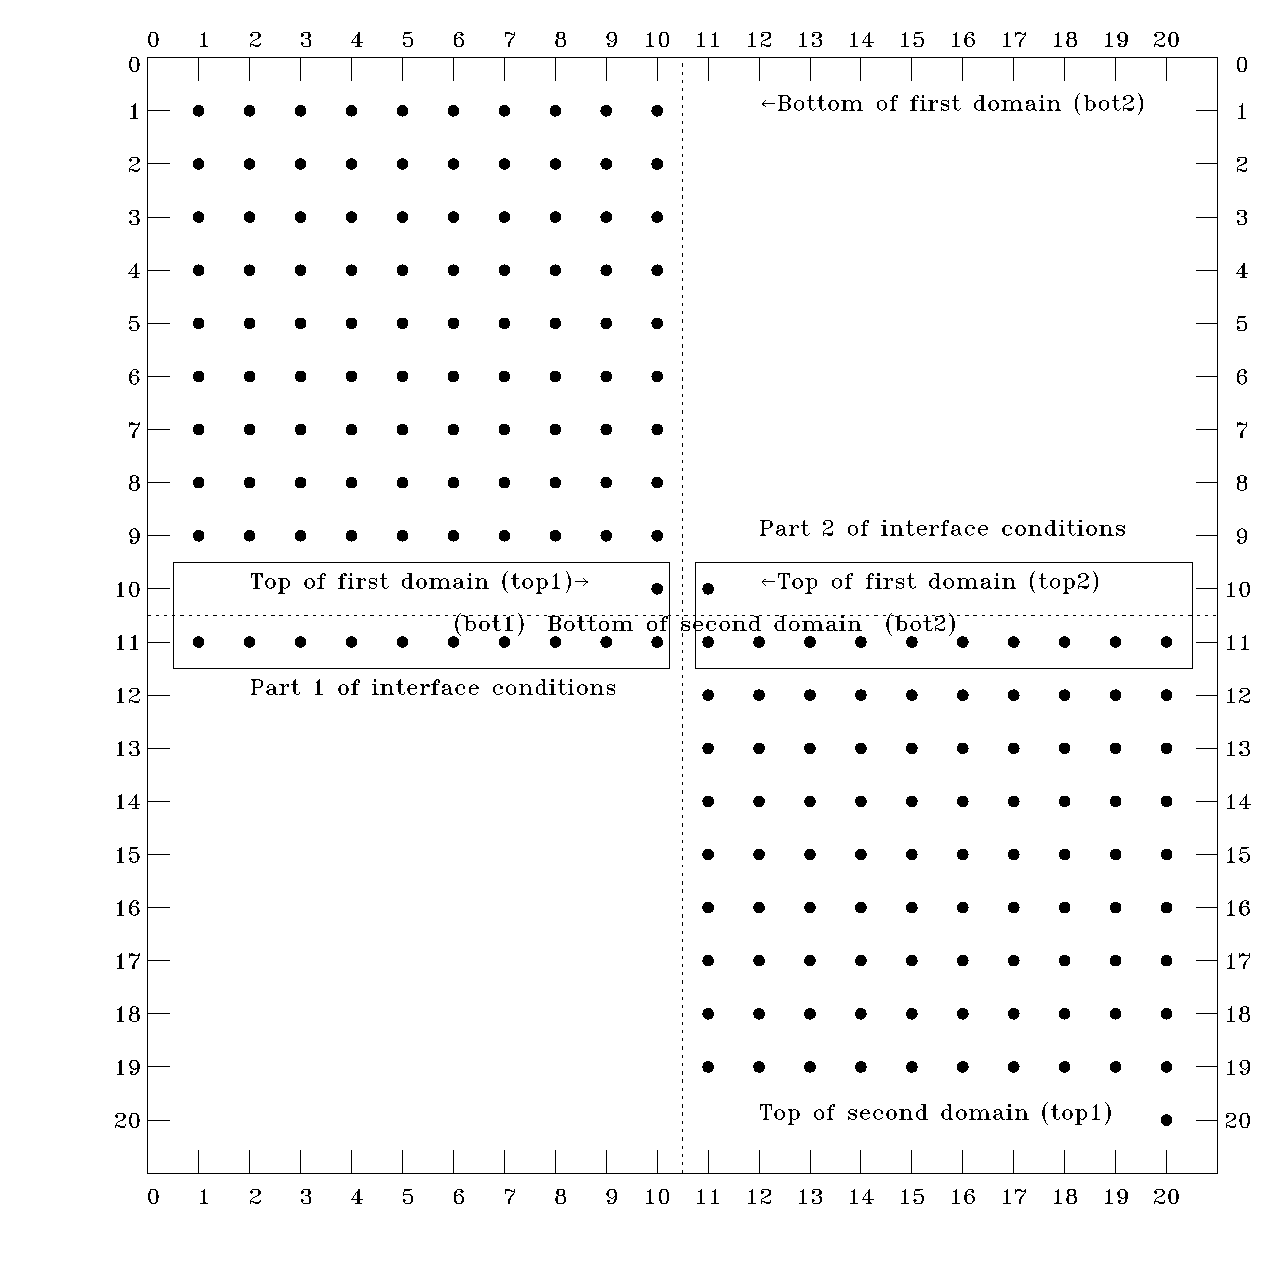
\includegraphics[width=0.8\linewidth]{fig/matrix_pedago.eps}
\caption{Example of discretized-operator matrix with two domains and
interface conditions.}
\label{matp}
\end{figure}

\subsection{Setting interface and boundary conditions}

At the interface of two domains we need to impose the continuity of the
functions and of their normal derivative (when the operators are of
second order). The conditions are imposed on the last grid point of the
lower domain and on the first grid point of the upper domain. To be
clear let us take an example of a 1D problem, where at some radius
$\zeta=\eta$ we impose

\[ f(\zeta_{\rm interf}^n) = f(\zeta_{\rm interf}^{n+1}) \andet f'(\zeta_{\rm
interf}^n) = f'(\zeta_{\rm interf}^{n+1})\]
where the prime is for the derivative. $n$ designates the lower domain
and $n+1$ the upper domain. Of course $\zeta_{\rm interf}^n=\zeta_{\rm
interf}^{n+1}=\eta$. The equation to be solved may be Laplace
equation for instance. In figure~\ref{matp} we display the structure of the
matrix using 20 grid points, with 10 points in each domain. We use the
strong formulation of the differential problem \cite[][]{RELP16}. On the
first line of the matrix we have, for instance, the boundary condition
at the bottom of the first domain. On row 10, the last grid point of the
first domain, we impose the continuity of the solution, so the first dot
is just "1" and the second dot is "-1". In the ESTER-nomenclature, the
"1" represents the first part of the interface condition while the "-1"
is the second part. Hence the "1" is inserted in the matrix via a {\tt
bc\_top1\_add} operation, while the "-1" is inserted in the matrix via a
{\tt bc\_top2\_add}  operation.

The second domain, in our example, starts at row 11 by the other
interface condition imposing the continuity of the derivative of the
solution. In the ESTER-nomenclature, the lower domain ($n-1$) part is
inserted by a {\tt bc\_bot1\_add} operation, while the actual domain $n$
condition need a {\tt bc\_bot2\_add} operation (see figure~\ref{matp}). In
row 20, we impose the ``surface" boundary condition saying $f(\zeta_{\rm
surf})=0$, so the dot is just a "1".


\subsection{Implementation of Newton's algorithm}

The construction of ESTER's models follows the following steps:

%\begin{tabular}{c}
%\hline
%\end{tabular}

\noindent -----------------------------------------------------------------------
\begin{enumerate}

\item Read the initial model or build it (only in 1D)
\item Build the Jacobian matrix
\item LU factorization of the Jacobian matrix
\item CGS solve (or refine) for the correction $\delta\vx$
\item Update $\vx$
\item recompute the RHS, $\vF(\vx_k)$ and the Jacobian matrix
\item Attempt a Conjugate Gradient Squared (CGS) solution to derive the new
$\delta\vx$ using the former LU matrices as a preconditionner. Namely,
if $L_k$ and $U_k$ are the factors of $\tens J_k$, the $k+1$ equation is
solved with the (split-preconditioned) CGS solver as

\[ J_k^{k+1}U_k\delta\vx_{k+1} = -L_k^{-1}\vF_{k+1}  \]
where the $J_k^{k+1}=L_k^{-1}\tens J_{k+1}U_k^{-1}$-matrix is almost
diagonal. If the convergence of this iterative method is less than say N
iterates, then the algorithm continues at step 5. N is chosen such that
the N iterations are faster than a LU factorization. If convergence is
not reached, then the algorithm continues on step 3

\item if $\|\delta\vx\|/\|\vx\|\leq$tolerance, then stop.
\end{enumerate}
\noindent -----------------------------------------------------------------------

\section{Modifying the equations}

Two kinds of modifications are conceivable: either to modify existing
equations or to add new equations coupled to the existing ones.

\subsection{Adding a new force or a heat source}

{\it Under construction}

\subsection{Adding a new equation and a new variable}

{\it Under construction}

\bigskip
\bigskip
The code is divided in several libraries. Each library implements one or
more classes designed to handle one particular aspect of the calculation.

\begin{itemize}
\item {\bf matrix}. Matrix algebra.

\item {\bf numdiff}. Implements Gauss-Legendre and multi-domain
Gauss-Lobatto numerical differentiation.

\item {\bf mapping}. Defines the mapping in spheroidal coordinates
$r(\zeta,\theta)$.

\item {\bf solver}. Resolution of systems of linear differential equations
in 2D.

\item {\bf physics}. Calculation of physical quantities (opacity,
equation of state, nuclear reaction rates).

\item {\bf star}. Provides objects and functions to calculate the
structure of a star in 1D and 2D.

\item {\bf global}. Definition of global variables, e.g. physical and mathematical constants.

\item {\bf graphics}. Provides graphical output through {\tt pgplot}.
\item {\bf parser}. Parsing of configuration files and command-line
arguments and file input/output.

\end{itemize} 


